% CCI v2 (Counterfactual Consistency Invariance) -- pipeline diagram, BLUE palette.
% Paper version: unified single-hue blue scheme (Tailwind "sky" ramp) + neutral
% slate input. Title nodes removed (the paper \caption serves that role).
% Compiles with pdflatex (MiKTeX). Standalone -> tight-cropped PDF.
\documentclass[tikz,border=6pt]{standalone}
\usepackage{amsmath}
\usepackage{amssymb}
\usepackage{bm}
\newcommand{\bth}{\bm{\theta}}   % bold theta, matches paper notation
\usetikzlibrary{
  positioning, arrows.meta, fit, backgrounds, calc,
  shadows.blur, decorations.pathreplacing, shapes.arrows, shapes.geometric
}

% ---- Unified blue palette (Tailwind sky ramp) + neutral slate input ----
\definecolor{inputgrey}{HTML}{64748B}     % slate-500  -- input (neutral, pre-method)
\definecolor{contribgreen}{HTML}{0EA5E9}  % sky-500    -- counterfactual generation
\definecolor{encblue}{HTML}{0284C7}       % sky-600    -- shared encoder
\definecolor{tempgold}{HTML}{0369A1}      % sky-700    -- logits / posterior
\definecolor{lossverm}{HTML}{0C4A6E}      % sky-900    -- objective / loss
\definecolor{inkdark}{HTML}{1F2937}
\definecolor{bandgrey}{HTML}{F3F4F6}

\begin{document}
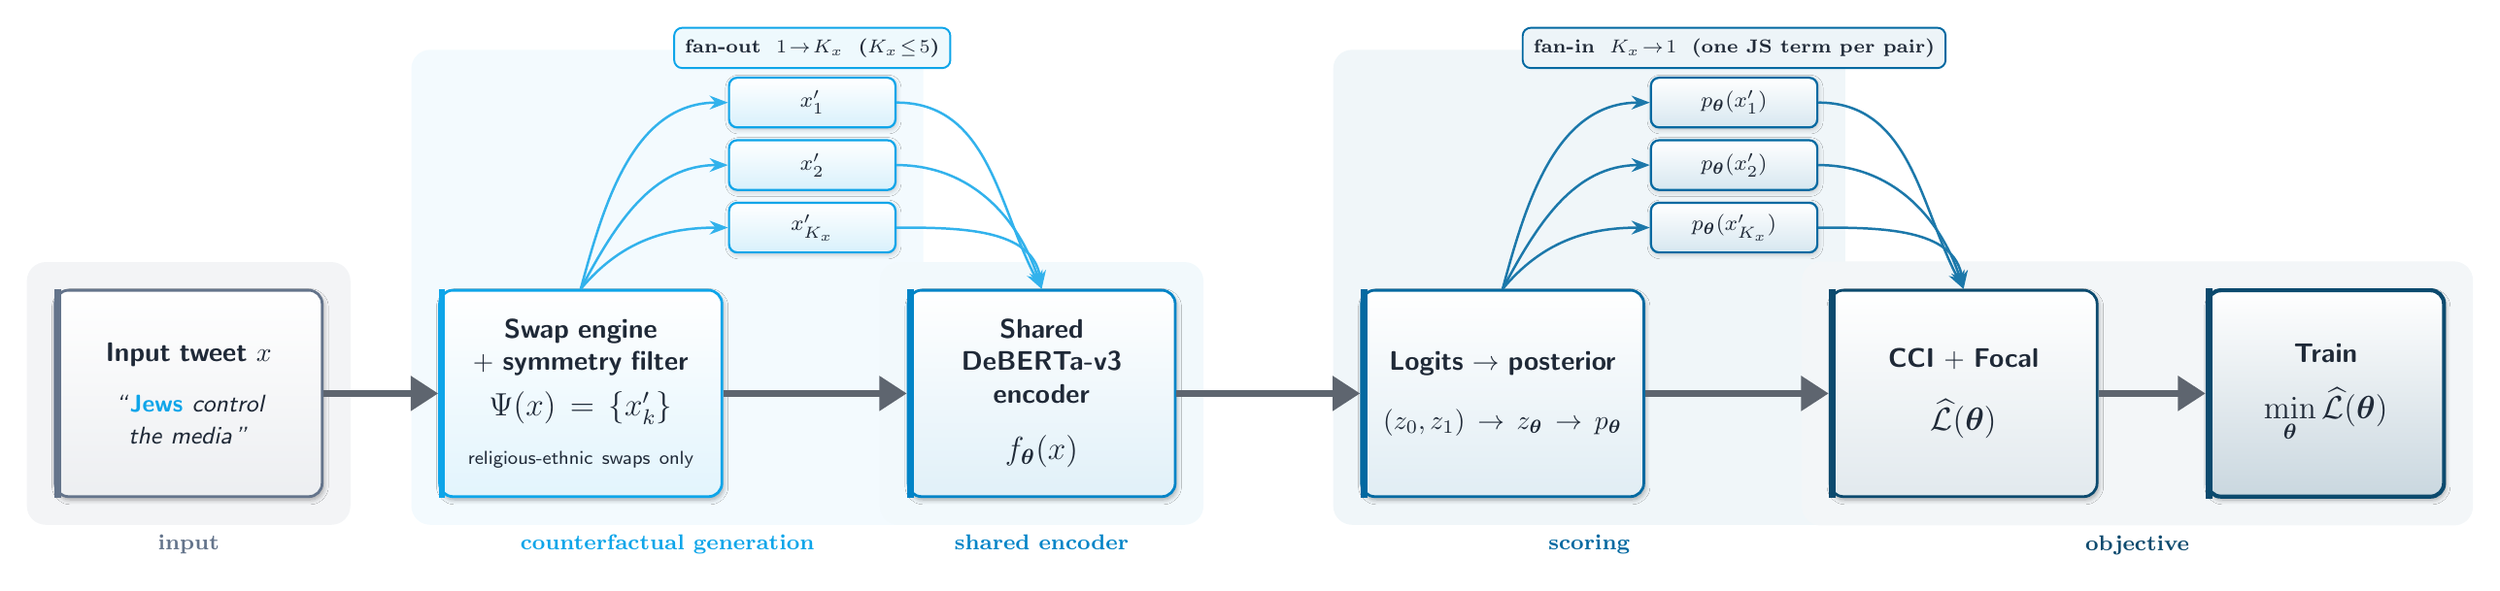
\begin{tikzpicture}[
  font=\sffamily,
  >={Stealth[round]},
  card/.style 2 args={
    rounded corners=5pt, draw=#1, line width=1pt,
    top color=white, bottom color=#1!12,
    blur shadow={shadow blur steps=6, shadow xshift=0.6pt,
                 shadow yshift=-1.2pt, shadow opacity=32},
    text=inkdark, align=center, inner sep=7pt,
    minimum height=27mm, text width=#2
  },
  accent/.style={line width=2.4pt, draw=#1},
  chip/.style={
    rounded corners=3pt, draw=#1, line width=0.8pt,
    top color=white, bottom color=#1!16, text=inkdark,
    inner sep=2.5pt, align=center, minimum height=6.5mm, text width=20mm,
    font=\footnotesize,
    blur shadow={shadow blur steps=4, shadow xshift=0.4pt,
                 shadow yshift=-0.7pt, shadow opacity=22}
  },
  note/.style={
    rounded corners=3pt, draw=#1, line width=0.7pt, fill=#1!7,
    text=inkdark, font=\scriptsize, inner sep=4pt, align=center
  },
  flow/.style={-{Triangle[length=3.6mm,width=4.4mm]},
               line width=2.4pt, draw=inkdark!72},
  fan/.style={-{Stealth[length=2.4mm]}, line width=0.9pt, draw=contribgreen!85},
  fin/.style={-{Stealth[length=2.4mm]}, line width=0.9pt, draw=tempgold!90},
]

% =====================================================================
%  MAIN ROW OF CARDS
% =====================================================================
\node[card={inputgrey}{30mm}] (inp) at (0,0) {
  \textbf{Input tweet $x$}\\[8pt]
  \itshape\small ``\,\textcolor{contribgreen}{\textbf{Jews}} control\\the media\,''
};

\node[card={contribgreen}{32mm}, right=15mm of inp] (swap) {
  \textbf{Swap engine}\\\textbf{$+$ symmetry filter}\\[5pt]
  {\large$\Psi(x)=\{x'_k\}$}\\[6pt]
  \scriptsize religious-ethnic swaps only
};

\node[card={encblue}{30mm}, right=24mm of swap] (enc) {
  \textbf{Shared}\\\textbf{DeBERTa-v3}\\\textbf{encoder}\\[9pt]
  {\large$f_{\bth}(x)$}
};

\node[card={tempgold}{32mm}, right=24mm of enc] (prob) {
  \textbf{Logits $\to$ posterior}\\[10pt]
  $(z_0,z_1)\,\to\, z_{\bth}\,\to\, p_{\bth}$
};

\node[card={lossverm}{30mm}, right=24mm of prob] (js) {
  \textbf{CCI $+$ Focal}\\[10pt]
  {\large$\widehat{\mathcal{L}}(\bth)$}
};

\node[card={lossverm}{26mm}, right=14mm of js,
      bottom color=lossverm!22, line width=1.5pt] (loss) {
  \textbf{Train}\\[9pt]
  {\large$\displaystyle\min_{\bth}\widehat{\mathcal{L}}(\bth)$}
};

\foreach \n/\c in {inp/inputgrey, swap/contribgreen, enc/encblue,
                   prob/tempgold, js/lossverm, loss/lossverm}{
  \draw[accent=\c] ([xshift=1.4pt]\n.north west) -- ([xshift=1.4pt]\n.south west);
}

% =====================================================================
%  MAIN FLOW ARROWS
% =====================================================================
\draw[flow] (inp)  -- (swap);
\draw[flow] (swap) -- (enc);
\draw[flow] (enc)  -- (prob);
\draw[flow] (prob) -- (js);
\draw[flow] (js)   -- (loss);

% =====================================================================
%  FAN-OUT (1 -> K) above the swap->encoder gap
% =====================================================================
\node[chip={contribgreen}, above=14mm of enc, xshift=-30mm, yshift=7mm] (cf1){$x'_1$};
\node[chip={contribgreen}, below=1.4mm of cf1] (cf2){$x'_2$};
\node[chip={contribgreen}, below=1.4mm of cf2] (cf3){$x'_{K_x}$};
\draw[fan] (swap.north) to[out=75,in=180] (cf1.west);
\draw[fan] (swap.north) to[out=62,in=180] (cf2.west);
\draw[fan] (swap.north) to[out=50,in=180] (cf3.west);
\draw[fan] (cf1.east) to[out=0,in=118] (enc.north);
\draw[fan] (cf2.east) to[out=0,in=108] (enc.north);
\draw[fan] (cf3.east) to[out=0,in=98]  (enc.north);
\node[note={contribgreen}, above=1mm of cf1, font=\scriptsize\bfseries]
  {fan-out\; $1\!\to\!K_x$ \;($K_x\!\le\!5$)};

% =====================================================================
%  FAN-IN (K -> 1) above the prob->js gap
% =====================================================================
\node[chip={tempgold}, above=14mm of js, xshift=-30mm, yshift=7mm] (p1){$p_{\bth}(x'_1)$};
\node[chip={tempgold}, below=1.4mm of p1] (p2){$p_{\bth}(x'_2)$};
\node[chip={tempgold}, below=1.4mm of p2] (p3){$p_{\bth}(x'_{K_x})$};
\draw[fin] (prob.north) to[out=75,in=180] (p1.west);
\draw[fin] (prob.north) to[out=62,in=180] (p2.west);
\draw[fin] (prob.north) to[out=50,in=180] (p3.west);
\draw[fin] (p1.east) to[out=0,in=118] (js.north);
\draw[fin] (p2.east) to[out=0,in=108] (js.north);
\draw[fin] (p3.east) to[out=0,in=98]  (js.north);
\node[note={tempgold}, above=1mm of p1, font=\scriptsize\bfseries]
  {fan-in\; $K_x\!\to\!1$ \;(one JS term per pair)};

% =====================================================================
%  PHASE-BAND BACKGROUNDS
% =====================================================================
\begin{scope}[on background layer]
  \node[fit=(inp), rounded corners=7pt, fill=bandgrey, inner sep=10pt,
        label={[font=\footnotesize\bfseries, text=inputgrey]below:input}] {};
  \node[fit=(swap)(cf1)(cf3), rounded corners=7pt, fill=contribgreen!5,
        inner sep=10pt,
        label={[font=\footnotesize\bfseries, text=contribgreen]below:counterfactual generation}] {};
  \node[fit=(enc), rounded corners=7pt, fill=encblue!5, inner sep=10pt,
        label={[font=\footnotesize\bfseries, text=encblue]below:shared encoder}] {};
  \node[fit=(prob)(p1)(p3), rounded corners=7pt, fill=tempgold!6, inner sep=10pt,
        label={[font=\footnotesize\bfseries, text=tempgold]below:scoring}] {};
  \node[fit=(js)(loss), rounded corners=7pt, fill=lossverm!5, inner sep=10pt,
        label={[font=\footnotesize\bfseries, text=lossverm]below:objective}] {};
\end{scope}

\end{tikzpicture}
\end{document}
